\documentclass[twocolumn]{article}
\usepackage{graphicx}
\usepackage{amsmath}
\usepackage{hyperref}
\usepackage{geometry}
\usepackage{algorithm}
\usepackage{algpseudocode}
\usepackage{titling}
\usepackage[
backend=biber,
style=numeric,
citestyle = numeric,
sorting=ynt
]{biblatex}

\addbibresource{ref.bib}

\geometry{a4paper, margin=1in}


\begin{document}

\twocolumn[{
    \begin{@twocolumnfalse}
    \begin{center}
        \rule{\linewidth}{0.5pt}    % 상단 가로선
        \vspace{0.2em}
        
        {\large COSE474-2024F: Final Project Report}\\[0.3em]
        {\large ``\textbf{Adapting CLIP for Personal Color Analysis}''}\\[0.2em]
        
        \rule{\linewidth}{0.5pt}    % 하단 가로선
        
        \vspace{0.4em}
        Hanjun Park
    \end{center}
    \vspace{1.5em}  % 제목과 본문 사이 간격
    \end{@twocolumnfalse}
}]

\vspace{1.5em}

\section{Introduction}
\textbf{Motivation}. Personal color analysis is a subjective yet impactful approach that helps individuals determine which color palettes suit their physical appearance best. Personal colors are typically divided into four categories—spring, summer, fall, and winter—based on physical characteristics. Traditionally, personal color analysis requires a trained professional, making it inaccessible to many. The motivation behind this project is to democratize personal color analysis by making it accessible to anyone with an AI-driven solution.

\textbf{Problem Definition}. The primary problem we address is whether a pre-trained model, specifically CLIP (Contrastive Language-Image Pretraining), can accurately classify personal colors into these four categories based solely on visual features. We also explore what modifications or tuning methods are needed to enhance CLIP's classification performance.

\textbf{Contribution}. The study explores several learning strategies, including zero-shot, fine-tuning, and prompt-based tuning, with a focus on identifying the most reliable method for personal color classification\cite{radford2021learning}. This research aims to democratize personal color analysis, making it accessible to a broader audience without requiring expert intervention.

\section{Related Works}
\textbf{CLIP.} CLIP is a powerful pre-trained vision-language model developed by Radford et al. \cite{radford2021learning}. It learns to associate images and text in a shared embedding space through contrastive learning. This property allows CLIP to perform well in zero-shot classification tasks, such as personal color classification, without extensive retraining. 

\textbf{Zero-shot Learning.} Zero-shot learning has gained significant attention due to its efficiency in leveraging pre-trained models for new tasks without requiring task-specific training data. In this context, CLIP's inherent ability to align visual and textual representations makes it particularly effective for zero-shot classification scenarios, including personal color categorization.

\textbf{Fine-tuning.} Fine-tuning is a common method to adapt pre-trained models for specific tasks by updating their weights. Fully fine-tuning all parameters of large models like CLIP can significantly improve performance for task-specific applications but is computationally intensive. To address this, LoRA adapts the model by introducing low-rank matrices, thereby reducing computational overhead while retaining adaptation effectiveness \cite{hu2021lora}.

\textbf{Prompt Tuning.} Prompt tuning is an approach to adapt pre-trained models by adding contextual prompts to their inputs, allowing them to perform better on specific tasks with minimal changes to the model's parameters. Prompt tuning techniques, such as CoCoOp (Conditional Context Optimization) and P-Tuning v2, modify the input prompts fed into CLIP to enhance its classification performance for specific categories \cite{zhou2022conditional, liu2021p}. These methods are particularly useful for adapting large pre-trained models like CLIP without incurring the computational costs of full fine-tuning.

\section{Methods}
\begin{figure}[h]
\centering
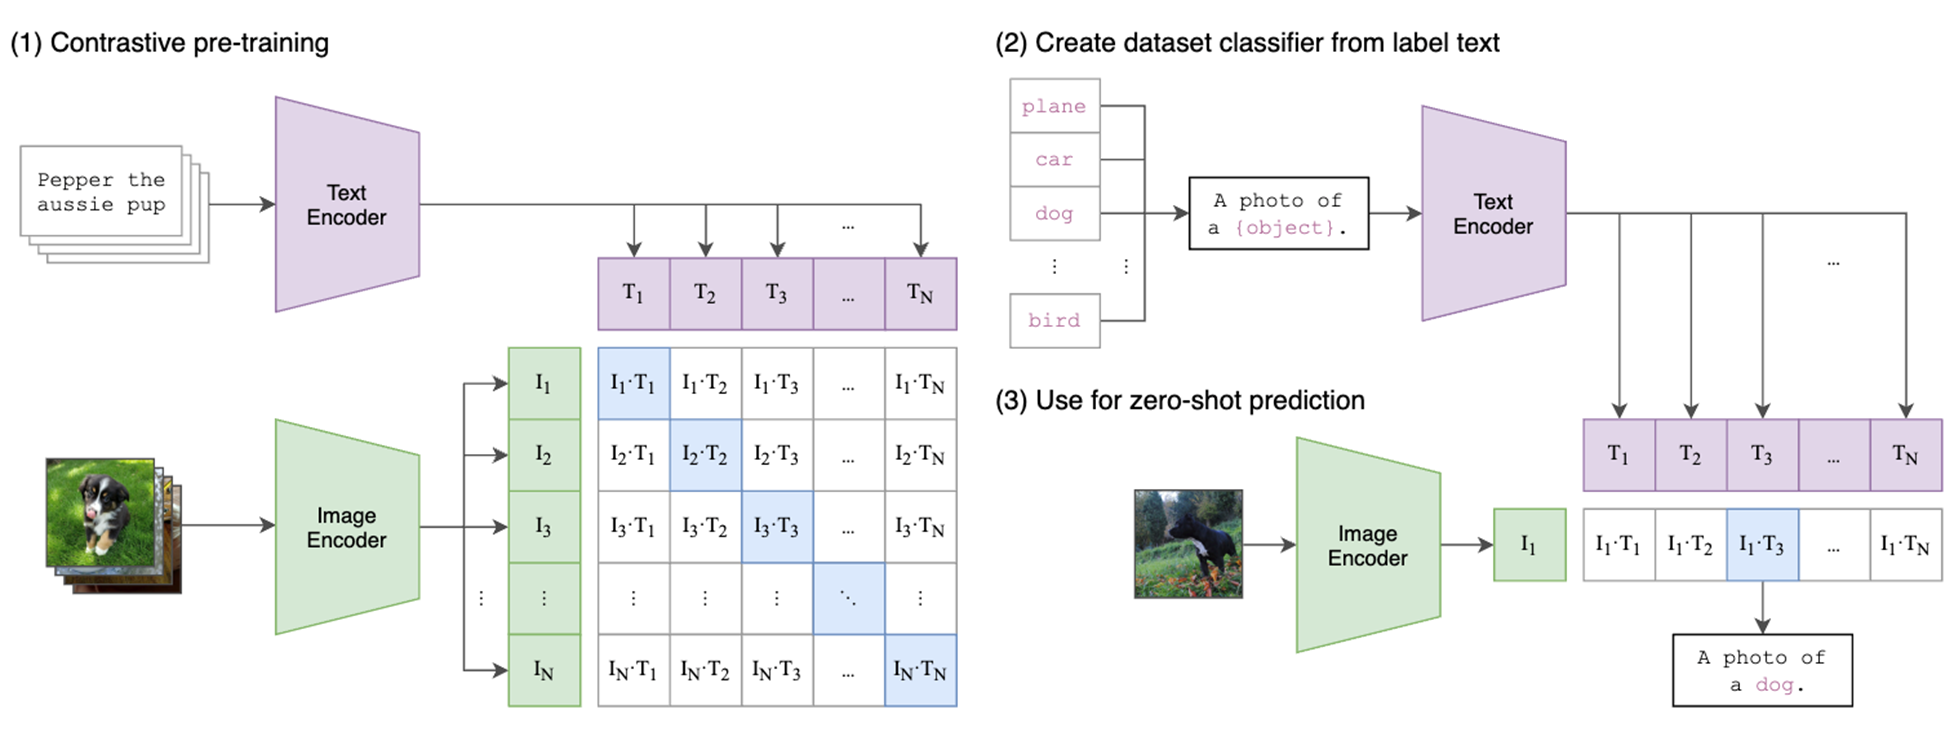
\includegraphics[width=0.45\textwidth]{Figure_Final_Project/CLIP_Arch.png}
\caption{The architecture of CLIP}
\label{fig:clip}
\end{figure}

This section describes the specific methods employed in this project. All methods build upon CLIP. Figure \ref{fig:clip} illustrates the core architecture of CLIP, which serves as the foundation for all tuning approaches used in this study. The significance of this study lies in its systematic exploration of multiple adaptation methods to evaluate CLIP's potential for domain-specific tasks like personal color classification.

\subsection{Fine-tuning}
\textbf{Fine-tuning} adapts the pre-trained CLIP model to the specific domain of personal color classification by updating its weights. Fully fine-tuning allows the model to learn domain-specific features, improving classification accuracy, though it is computationally intensive and risks overfitting on smaller datasets. For this experiment, we trained the model for 10 epochs, observing the highest performance during this period. This approach demonstrated CLIP's ability to adapt to fine-grained, visually subjective tasks through complete parameter updates. The process of fine-tuning is detailed in Algorithm \ref{alg:finetuning}.

\begin{algorithm}
\caption{Fine-tuning CLIP}
\label{alg:finetuning}
\begin{algorithmic}[1]
\Require CLIP visual encoder $f_V$, classifier $W_{\text{cls}}$
\For{batch $(x, y) \in D$}
    \State Extract features $v = f_V(x)$
    \State Compute logits $l = W_{\text{cls}}(v)$
    \State Update $f_V$ with learning rate $\eta_1$
    \State Update $W_{\text{cls}}$ with learning rate $\eta_2$
\EndFor
\State \Return Fine-tuned $f_V, W_{\text{cls}}$
\end{algorithmic}
\end{algorithm}

\textbf{LoRA-based Fine-tuning}.
LoRA (Low-Rank Adaptation) is a parameter-efficient technique that fine-tunes large pre-trained models by introducing low-rank matrices, reducing computational costs while retaining adaptation effectiveness. In this project, LoRA was implemented within CLIP's vision transformer blocks by introducing rank-4 projection layers, allowing the model to capture domain-specific features while maintaining computational efficiency. The LoRA-based fine-tuning process is detailed in Algorithm \ref{alg:lora}.

\begin{algorithm}
\caption{LoRA for CLIP}
\label{alg:lora}
\begin{algorithmic}[1]
\Require CLIP visual encoder $f_V$, LoRA layers $\{L_i\}_{i=1}^{12}$
\For{batch $(x, y) \in D$}
    \State Extract features $v = f_V(x)$
    \For{each $L_i$}
        \State $v = v + 0.1 \cdot W_{\text{up}}(W_{\text{down}}(v))$
    \EndFor
    \State Update LoRA parameters using gradient descent
\EndFor
\State \Return Optimized $\{L_i\}_{i=1}^{12}$
\end{algorithmic}
\end{algorithm}

\subsection{Prompt Tuning}
\textbf{CoCoOp.} Conditional Context Optimization extends CLIP's flexibility by dynamically generating prompts conditioned on input images. In this study, CoCoOp employed a meta-network to generate context embeddings tailored to personal color categories. These dynamic prompts allowed the model to better align visual and textual features without altering CLIP's core architecture. The CoCoOp tuning procedure is described in Algorithm \ref{alg:cocoop}.

\begin{algorithm}
\caption{Conditional Prompt Learning (CoCoOp)}
\label{alg:cocoop}
\begin{algorithmic}[1]
\Require CLIP model, learnable context $C$, meta-network $M_\theta$
\For{batch $(x, y) \in D$}
    \State Generate context features $c = M_\theta(C)$
    \State Extract image and text features $f_I, f_T$
    \State Compute logits $l = 100 \cdot f_I f_T^T$
    \State Update $C, M_\theta$ using gradient descent
\EndFor
\State \Return Optimized $C, M_\theta$
\end{algorithmic}
\end{algorithm}


\textbf{P-Tuning v2.} Prompt tuning modifies input prompts to better align CLIP's pre-trained embeddings with the task-specific requirements. For this project, P-Tuning v2 introduced learnable prompt embeddings to adapt to the nuanced characteristics of personal color classification. These embeddings were trained using backpropagation while keeping the CLIP parameters frozen, minimizing computational overhead. The P-Tuning v2 prompt tuning procedure is described in Algorithm \ref{alg:ptuning}.

\begin{algorithm}
\caption{P-tuning v2 for CLIP}
\label{alg:ptuning}
\begin{algorithmic}[1]
\Require Pre-trained CLIP visual encoder $f_V$, prompt encoder $P_\theta$
\For{batch $(x, y) \in D$}
    \State Extract features $v = f_V(x)$
    \State Generate prompted features $z = P_\theta(v)$
    \State Compute cross-entropy loss $\mathcal{L}_{\text{CE}}$
    \State Update $P_\theta$ using gradient descent
\EndFor
\State \Return Optimized $P_\theta$
\end{algorithmic}
\end{algorithm}


\subsection{Evaluation Metrics}
We evaluated our methods using two key metrics: accuracy and recall. The overall classification accuracy serves as our primary metric, calculated as:
\begin{equation}
\text{Accuracy} = \frac{\text{Number of correct predictions}}{\text{Total number of predictions}}
\end{equation}
Additionally, we computed the recall metric for each season category:
\begin{equation}
\text{Recall} = \frac{\text{True Positives}}{\text{True Positives + False Negatives}}
\end{equation}
These metrics were chosen to assess both the overall performance and the ability to correctly identify specific seasonal color types, which is crucial for the subjective nature of personal color analysis.

\begin{table*}[t]
\centering
\begin{tabular}{|c|c|c|c|c|}
\hline
\textbf{Method} & \textbf{Accuracy} & \textbf{Precision} & \textbf{Recall} & \textbf{F1-Score} \\
\hline
Zero-shot    & 22.31 & 22.00 & 24.00 & 19.00 \\
Fine-tuning  & 54.22 & 52.00 & 52.00 & 52.00 \\
LoRA         & 40.34 & 39.00 & 40.00 & 38.00 \\
CoCoOp       & 21.99 & 18.00 & 24.00 & 19.00 \\
P-Tuning v2  & 45.78 & 49.00 & 46.00 & 44.00 \\
\hline
\end{tabular}
\caption{Quantitative results of various tuning methods for personal color classification (all in percentages).}
\label{tab:quant_results}
\end{table*}

\section{Experiments}
\textbf{Dataset}
The dataset used in this study consists of 6,000 labeled images across four personal color categories: spring, summer, fall, and winter. The images were sourced from the Deep-Armocromia repository \cite{stacchiodeep} and Roboflow. Each category comprises 1,200 training images and 300 test images. The images were preprocessed to match CLIP's input requirements, including resizing to $224\times224$ pixels.

\textbf{Computing Resources}
All experiments were conducted using Google Colab Pro with an NVIDIA A100 GPU. The use of high-performance GPU resources allowed for efficient training and inference.

\textbf{Experimental Design}
The experiments were designed to evaluate the effectiveness of various tuning methods for personal color classification:

\begin{itemize}
\item \textbf{Baseline}: Zero-shot learning using the pre-trained CLIP model.
\item \textbf{Fine-tuning}: Fully fine-tuning CLIP and Low-Rank Adaptation for the classification task.
\item \textbf{Prompt Tuning}: Using CoCoOp and P-Tuning v2 for dynamic and learnable prompt tuning.
\end{itemize}

The primary goal was to identify which method best captures the subtle visual features necessary for accurate personal color classification.

\subsection{Quantitative Results}
Table \ref{tab:quant_results} summarizes the accuracy, recall, and other metrics for each method. Fine-tuning achieved the highest accuracy (54.2\%), followed by P-Tuning v2 (45.8\%) and LoRA (40.3\%).

Figure \ref{fig:performance_comparison} visualizes the performance comparison across methods.

\begin{figure}[h]
\centering
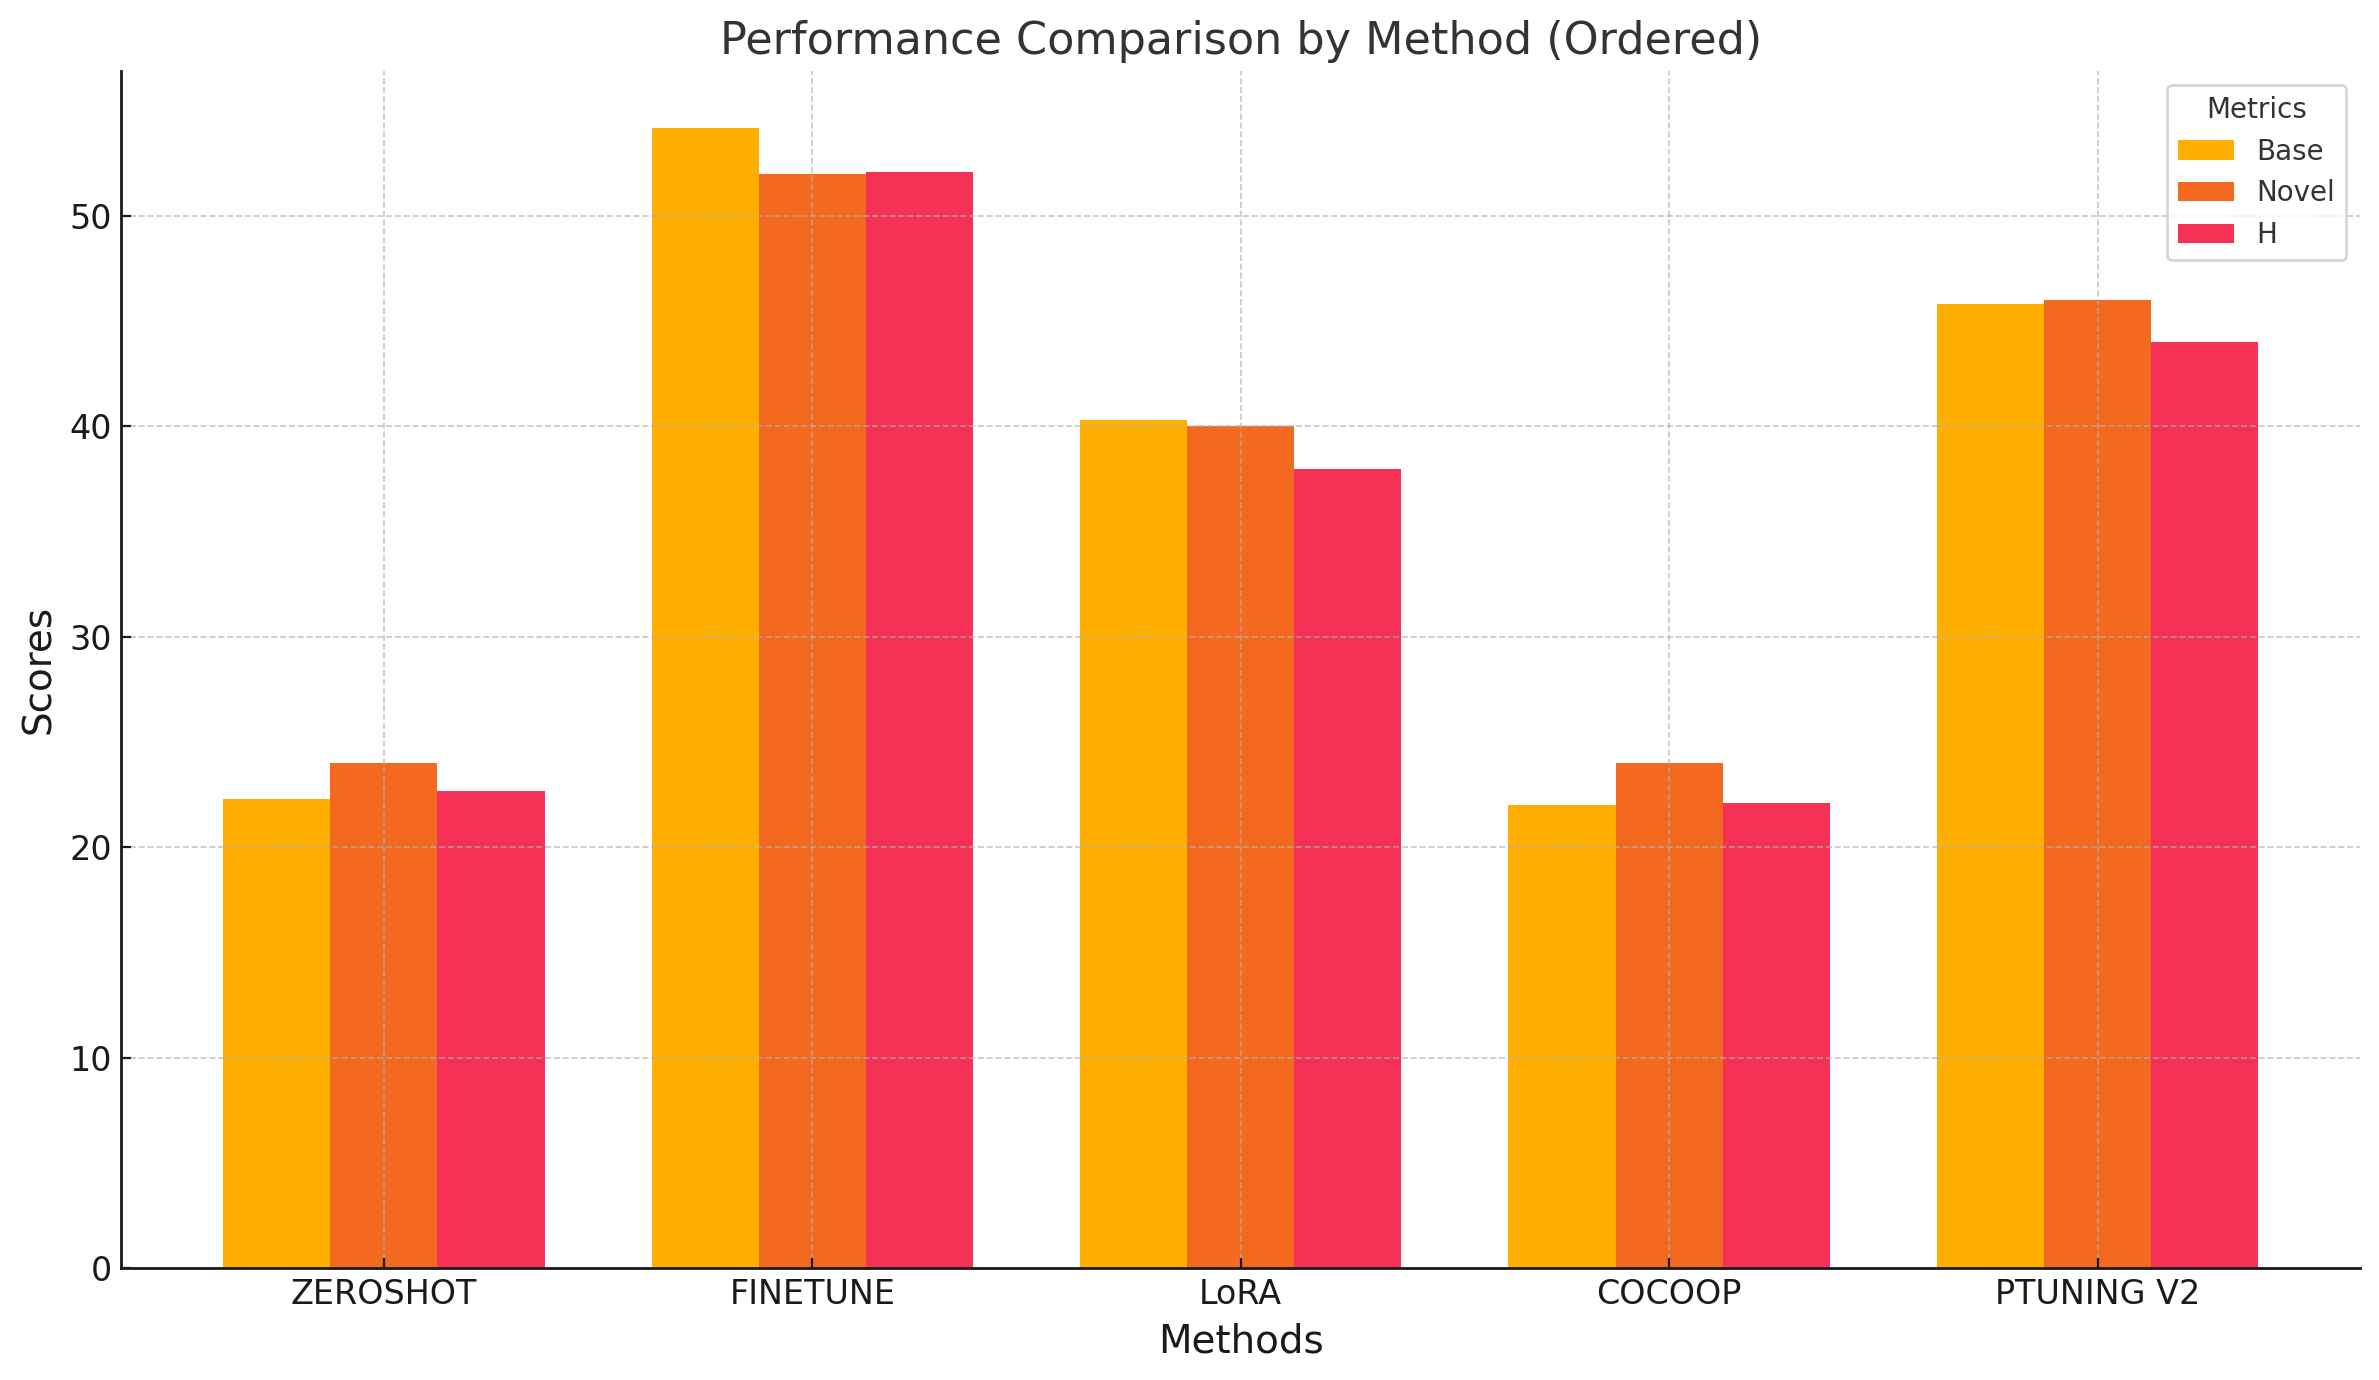
\includegraphics[width=0.45\textwidth]{Figure_Final_Project/DL_Project_chart.png}
\caption{Performance comparison of tuning methods based on accuracy and recall.}
\label{fig:performance_comparison}
\end{figure}

\subsection{Qualitative Results}
Qualitative analysis revealed that fine-tuning produced the most consistent predictions across all color categories, accurately distinguishing subtle differences in skin tones and lighting conditions. P-Tuning v2 also performed well but occasionally misclassified edge cases. Zero-shot learning and CoCoOp showed limited effectiveness, often failing to generalize across diverse inputs.

\subsection{Discussion}
Fine-tuning proved highly effective, enabling CLIP to adapt its generalist architecture for fine-grained tasks like personal color classification.\cite{wei2023improving} Remarkably, the fine-tuned CLIP achieved accuracy comparable to the state-of-the-art FaRL64 (55.4\%) on the Armocromia dataset,\cite{stacchiodeep} highlighting its potential for visual feature-based classification without requiring domain-specific pre-training.

In contrast, CoCoOp struggled due to its reliance on dynamic prompt generation,\cite{zhou2022conditional} limiting its ability to capture fine-grained features. While P-Tuning v2 and LoRA offered computationally efficient alternatives.\cite{hu2021lora}\cite{liu2021p}

This comparison underscores fine-tuning's capability to transform general-purpose models like CLIP into competitive tools for specialized tasks, bridging the gap with state-of-the-art methods.


\section{Future Directions}

To further enhance the model's capabilities, future efforts could focus on incorporating datasets with broader diversity in skin tones, lighting conditions, and cultural contexts, which would improve the model's generalization and robustness. Additionally, combining the strengths of fine-tuning and prompt-tuning approaches to develop hybrid models could also optimize both performance and computational efficiency. 

\nocite{*}
\printbibliography
\end{document}

